\documentclass[border=6pt]{standalone}
\usepackage{fontspec}
\usepackage[sfdefault,lining]{FiraSans}
\usepackage{pgfplots}
\usepgfplotslibrary{groupplots}
\pgfplotsset{compat=1.18}
\definecolor{tsnavy}{HTML}{1A2E4F}\definecolor{tsred}{HTML}{A6252D}\definecolor{tsink}{HTML}{1F2430}
\definecolor{tsgrey}{HTML}{5F6B7C}\definecolor{tsmuted}{HTML}{A7B2C2}\definecolor{tsline}{HTML}{D6DCE5}
\definecolor{cRepair}{HTML}{1B7F9E}\definecolor{cControl}{HTML}{C98A2B}
\definecolor{cVanOurs}{HTML}{F2C3C6}\definecolor{cVanPaper}{HTML}{8AA4CC}
\pgfplotsset{rd/.style={axis lines*=left, ymajorgrids, grid style={tsline,line width=0.4pt},
  axis line style={tsgrey,line width=0.5pt}, major tick style={draw=none},
  tick label style={font=\small,text=tsgrey,/pgf/number format/assume math mode=true}, label style={font=\small,text=tsink},
  title style={font=\bfseries\color{tsnavy}},
  legend style={draw=none,fill=none,font=\small,text=tsink,/tikz/every even column/.append style={column sep=10pt}},
  legend cell align=left, every axis plot/.append style={line width=0.5pt}}}
\begin{document}
\pagecolor{white}
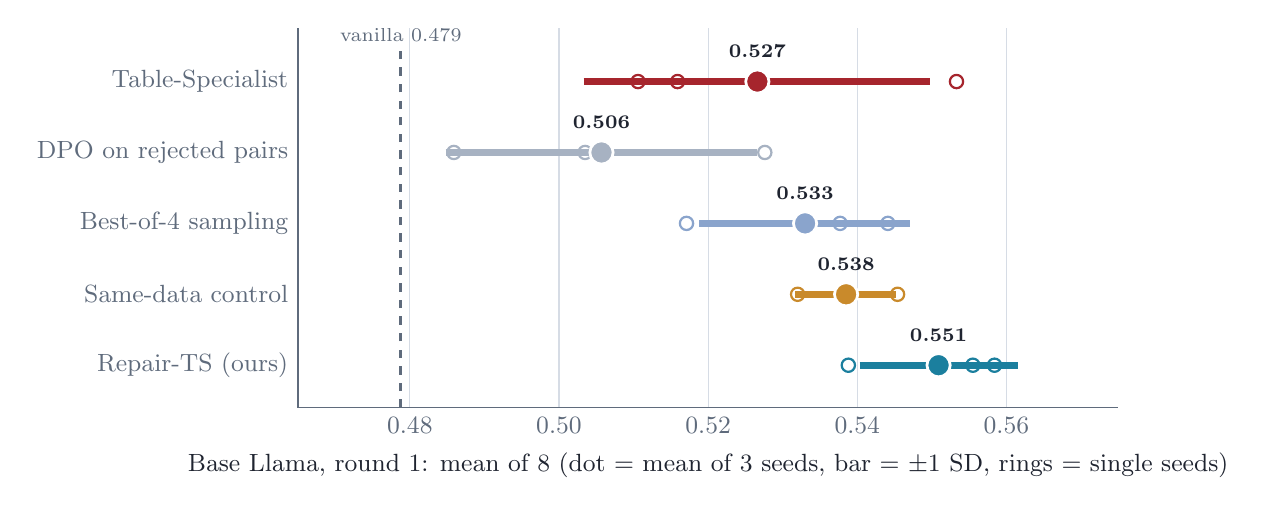
\begin{tikzpicture}
\begin{axis}[rd, ymajorgrids=false, xmajorgrids, width=12cm, height=6.4cm,
  xmin=0.465, xmax=0.575, ymin=-0.6, ymax=4.75, ytick={0,...,4}, yticklabels={Repair-TS (ours),Same-data control,Best-of-4 sampling,DPO on rejected pairs,Table-Specialist},
  xlabel={Base Llama, round 1: mean of 8 (dot = mean of 3 seeds, bar = $\pm$1 SD, rings = single seeds)},
  scaled x ticks=false, x tick label style={/pgf/number format/.cd,fixed,fixed zerofill,precision=2},
  xtick={0.48,0.50,...,0.56}]
\draw[tsgrey,dashed,line width=1pt] (axis cs:0.4788,-0.6) -- (axis cs:0.4788,4.45);
\node[font=\scriptsize,text=tsgrey,anchor=south] at (axis cs:0.4788,4.42) {vanilla 0.479};
\draw[cRepair,line width=2.6pt] (axis cs:0.5403,0) -- (axis cs:0.5615,0);
\addplot[only marks,mark=o,mark size=2.4pt,cRepair,line width=0.8pt] coordinates {(0.5388,0) (0.5584,0) (0.5555,0)};
\addplot[only marks,mark=*,mark size=4.2pt,cRepair,mark options={draw=white,line width=1pt}] coordinates {(0.5509,0)};
\node[font=\scriptsize\bfseries,text=tsink,anchor=south] at (axis cs:0.5509,0) [yshift=5pt] {0.551};
\draw[cControl,line width=2.6pt] (axis cs:0.5317,1) -- (axis cs:0.5452,1);
\addplot[only marks,mark=o,mark size=2.4pt,cControl,line width=0.8pt] coordinates {(0.5320,1) (0.5454,1) (0.5380,1)};
\addplot[only marks,mark=*,mark size=4.2pt,cControl,mark options={draw=white,line width=1pt}] coordinates {(0.5385,1)};
\node[font=\scriptsize\bfseries,text=tsink,anchor=south] at (axis cs:0.5385,1) [yshift=5pt] {0.538};
\draw[cVanPaper,line width=2.6pt] (axis cs:0.5188,2) -- (axis cs:0.5471,2);
\addplot[only marks,mark=o,mark size=2.4pt,cVanPaper,line width=0.8pt] coordinates {(0.5171,2) (0.5441,2) (0.5377,2)};
\addplot[only marks,mark=*,mark size=4.2pt,cVanPaper,mark options={draw=white,line width=1pt}] coordinates {(0.5330,2)};
\node[font=\scriptsize\bfseries,text=tsink,anchor=south] at (axis cs:0.5330,2) [yshift=5pt] {0.533};
\draw[tsmuted,line width=2.6pt] (axis cs:0.4848,3) -- (axis cs:0.5266,3);
\addplot[only marks,mark=o,mark size=2.4pt,tsmuted,line width=0.8pt] coordinates {(0.4859,3) (0.5276,3) (0.5035,3)};
\addplot[only marks,mark=*,mark size=4.2pt,tsmuted,mark options={draw=white,line width=1pt}] coordinates {(0.5057,3)};
\node[font=\scriptsize\bfseries,text=tsink,anchor=south] at (axis cs:0.5057,3) [yshift=5pt] {0.506};
\draw[tsred,line width=2.6pt] (axis cs:0.5033,4) -- (axis cs:0.5498,4);
\addplot[only marks,mark=o,mark size=2.4pt,tsred,line width=0.8pt] coordinates {(0.5106,4) (0.5159,4) (0.5533,4)};
\addplot[only marks,mark=*,mark size=4.2pt,tsred,mark options={draw=white,line width=1pt}] coordinates {(0.5266,4)};
\node[font=\scriptsize\bfseries,text=tsink,anchor=south] at (axis cs:0.5266,4) [yshift=5pt] {0.527};
\end{axis}
\end{tikzpicture}
\end{document}
